\section*{Math 202a - HW3 - Dan Davison - \texttt{ddavison@berkeley.edu}}

Homework 3 was quite a bit tougher, owing to exercise 2.12 (no countable sigma-algebras). A lot of students didn't finish 2.18 (stochastic arithmetic) but those who did got most of the ideas, at least, right. By the way, since 2.18 was so long, we assigned triple credit for it this week.

One common approach to 2.12 involved choosing an arbitrary sequence of distinct measurable sets $A_n$ and mapping binary sequences $k_n$ into something like $\bigcup_n B_n$ where $B_n = A_n$ if $k_n = 1$ and $B_n = A_n^c$ else. A nice exercise would be to show that this does not work if the $A_n$ are, for example, a chain: $A_n \subseteq A_{n+1}$. The idea here isn't bad, but one needs to be very careful in how one chooses the $A_n$.

So it's tempting to consider the sets $A_\omega = \bigcap \{B: \omega \in B\}$, but one immediately runs into two problems: the $A_\omega$ may not be measurable, and of course the map $\omega \mapsto A_\omega$ is not injective if $\Omega = \mathbb Z$ and the measurable sets are generated by sets of the form $\{-n, n\}$ (why not?) By imposing an equivalence relation on $\Omega$ many of you overcame the latter problem. The former is more subtle: the problem asks you to show that the $\sigma$-algebra has cardinality at least that of $\mathbb R$, but many of you said that if this failed then the $\sigma$-algebra was in bijection with $\mathbb N$ (which implies that $A_\omega$ is measurable), and so fell victim to Cohen's forcing theorem: it is NOT true that every uncountable set has cardinality at least that of $\mathbb R$ unless one makes some very special hypotheses on the underlying logical system we are using!!

I wrote a lot more about my thoughts about 2.12, including a rather combinatorial proof that I cooked up, at this blog post: https://backus.home.blog/2020/09/28/boolean-algebras-and-probability/ -- really, the problem that it's so hard is that it has nothing to do with measure theory and everything to do with infinite combinatorics. I use the word "standard Borel space" a few times, but whenever I say that you can just think $\mathbb R$.

Problem 2.4: This was fine for the most part. However, a common mistake on part (b) (the counterexample) was to present a sequence of sigma-algebras that *are not defined on a common space* Omega. Most of the mistakes of this type were easily fixable, but still a common mistake.

Problem 2.5: I think everyone verified part (a) just fine. Most, if not all, of the trouble was in part (b). The meat of the solution was in verifying that script{A} is a field itself. Verifying closure under complements seemed to be the biggest problem. Once you take your arbitrary set A = \cup_i \cap_j A_{i,j} \in \script{A}, you find the complement by applying a DeMorgan’s law. But then your left with A^c = \cap_i \cup_j A_{i,j}^c, which is not clearly in our family of sets due to a possible disjointedness issue. To fix this, one must express \cup_{j=1} A_{i,j}^c in the form given in the hint in Billingsley. This gives A^c as a unions of finitely many *disjoint* intersections. Sorry that this is a mouthful, but I think that’s where most of the confusion on this problem came from.

\begin{enumerate}
\item~\\
  \begin{mdframed}
    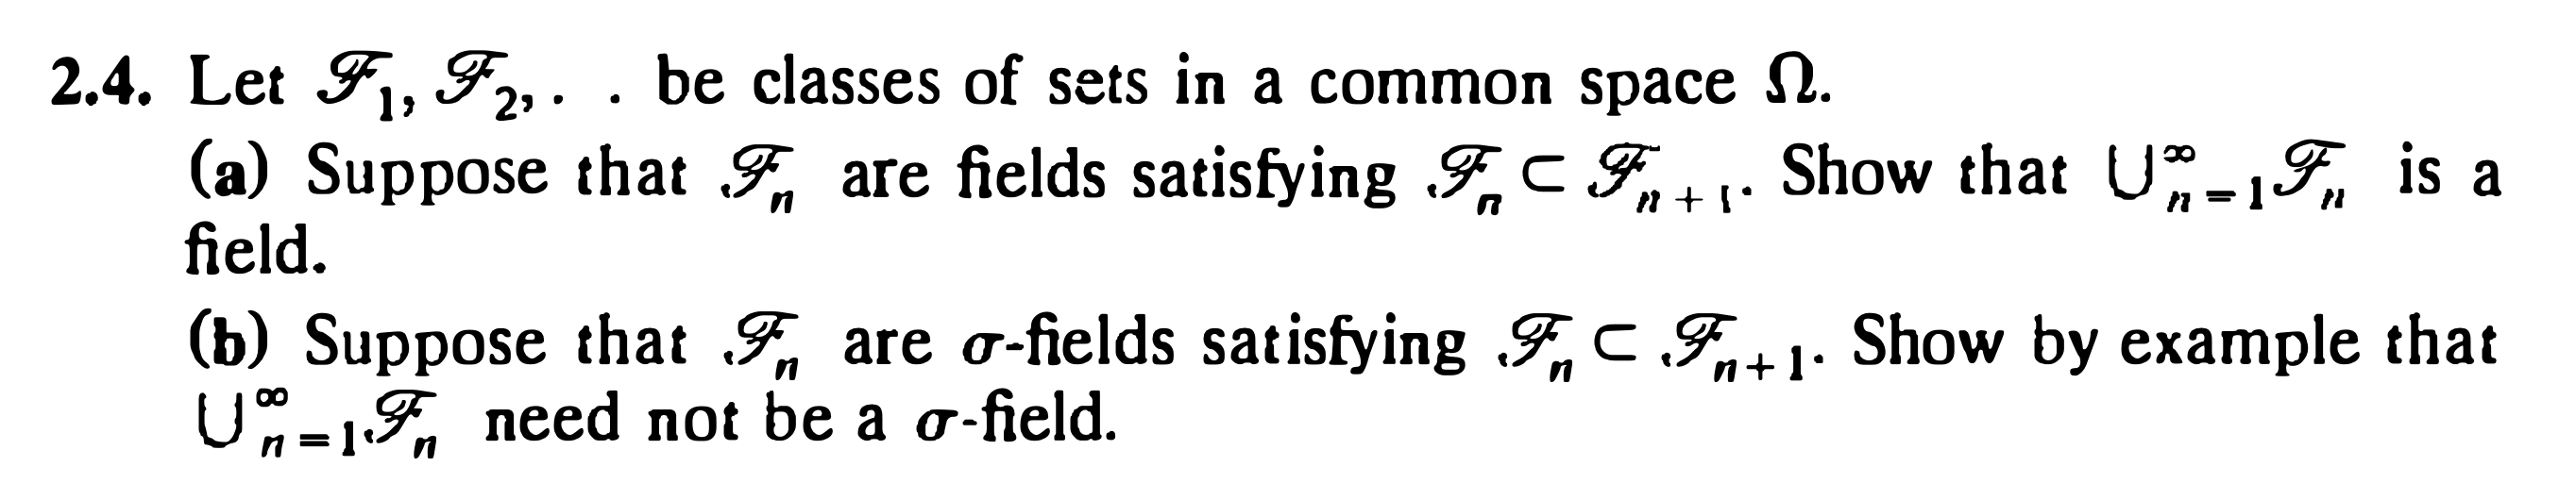
\includegraphics[width=400pt]{img/analysis--berkeley-202a-hw-e32d.png}
  \end{mdframed}
  \begin{enumerate}[label=(\alph*)]
  \item
    \begin{claim*}[countable union of algebras is an algebra]
      Let $\ms F_1, \ms F_2, \ldots$ be algebras on $\Omega$ (collections of events).
      Then $\bigcup_{n=1}^\infty \ms{F}_n$ is an algebra.
    \end{claim*}

    \begin{proof}
      Let $\ms F = \bigcup_{n=1}^\infty \ms F_n$. We must show that
      \begin{enumerate}
      \item $\Omega \in \ms F$ \\
        {\bf Proof:} $\ms F_1$ is an algebra, therefore $\Omega \in \ms F_1$, therefore $\Omega \in \ms F$.
      \item If $A \in \ms F$ then $A^c \in \ms F$ \\
        {\bf Proof:} If $A \in \ms F$ then $A \in F_n$ for some $n$. Therefore $A^c \in \ms F_n$. Therefore $A^c \in \ms F$.
      \item If $A, B \in \ms F$ then $A \cup B \in \ms F$ \\
        {\bf Proof:} If $A, B \in \ms F$ then for some $m$ and $n$ we have $A \in \ms F_m$ and $B \in \ms F_n$.
        Suppose $m = n$. Then $A \cup B \in \ms F_m$, therefore $A \cup B \in \ms F$. Alternatively
        suppose $m \neq n$. Then either $\ms F_m \subset \ms F_n$ or $\ms F_n \subset \ms F_m$. Suppose without
        loss of generality that $\ms F_m \subset \ms F_n$. Then $A, B \in \ms F_n$,
        therefore $A \cup B \in \ms F_n$, therefore $A \cup B \in \ms F$.
      \end{enumerate}
    \end{proof}
  \item
    \begin{claim*}[countable union of nested $\sigma$-algebras may not be a $\sigma$-algebra]
      Let $\ms F_1, \ms F_2, \ldots$ be $\sigma$-algebras satisfying $\ms F_n \subset \ms F_{n+1}$.
      Then $\bigcup_{n=1}^\infty \ms{F}_n$ may not be a $\sigma$-algebra.
    \end{claim*}

    \begin{proof}
      Let $\Omega = (0, 1]$, let $\ms A_n$ be the set of rank-$n$ dyadic intervals in $[0, 1]$ and
      define $\ms F_n = \sigma(\ms A_n)$, the $\sigma$-algebra generated by $\ms F_n$. Then for example we have
      \begin{align*}
        \ms F_1 &= \Big\{\emptyset,
                  (0, .5], (.5, 1],
                  (0, 1]
                  \Big\} \\
                  % \ms F_2 &= \Big\{\emptyset,
                  % (0, .25], (.25, .5], (.5, .75], (.75, 1],
                  % (0, .5], (.5, 1],
                  % (0, .75], (.25, .75],
                  % (0, 1],
                  % (.25, 1]
                  % \Big\}
      \end{align*}
      Note however that $(1 - 2^{-n}, 1] \in \ms F_n$ and that $\bigcap_{n=1}^\infty (1 - 2^{-n}, 1] = \{1\}$.
      Therefore if $\bigcup_{n=1}^\infty \ms F_n$ is a $\sigma$-algebra
      then $\{1\} \in \bigcup_{n=1}^\infty \ms F_n$.

      But $\{1\}$ is not a dyadic interval, therefore there is no $n$ for which $\{1\} \in \ms A_n$.
      Furthermore there is no $n$ for which $\{1\} \in \sigma(\ms A_n)$ (justification below).

      Therefore $\{1\} \notin \bigcup_{n=1}^\infty \ms F_n$ and so $\bigcup_{n=1}^\infty \ms F_n$ is not a $\sigma$-algebra.

      ~\\
      \textbf{Justification that there is no $n$ for which $\{1\} \in \sigma(\ms A_n)$:}

      By definition, $\sigma(\ms A_n)$ is the intersection of all $\sigma$-algebras that include $\ms A_n$.
      Suppose $\{1\} \in \sigma(\ms A_n)$. Now form a new class of sets $\sigma^*(\ms A_n)$ by removing
      from $\sigma(\ms A_n)$ every set that contains $1$ as an isolated point, and its complement. We claim
      that $\sigma^*(\ms A_n)$ is a $\sigma$-algebra. Note that none of the removed sets were in $\ms A_n$
      (since they are not dyadic intervals). But
      then $\ms A_n \subseteq \sigma^*(\ms A_n) \subset \sigma(\ms A_n)$ which contradicts the definition
      of $\sigma(\ms A_n)$. Therefore $\{1\} \notin \sigma(\ms A_n)$.
    \end{proof}
  \end{enumerate}

  \newpage
\item~\\
  \begin{mdframed}
    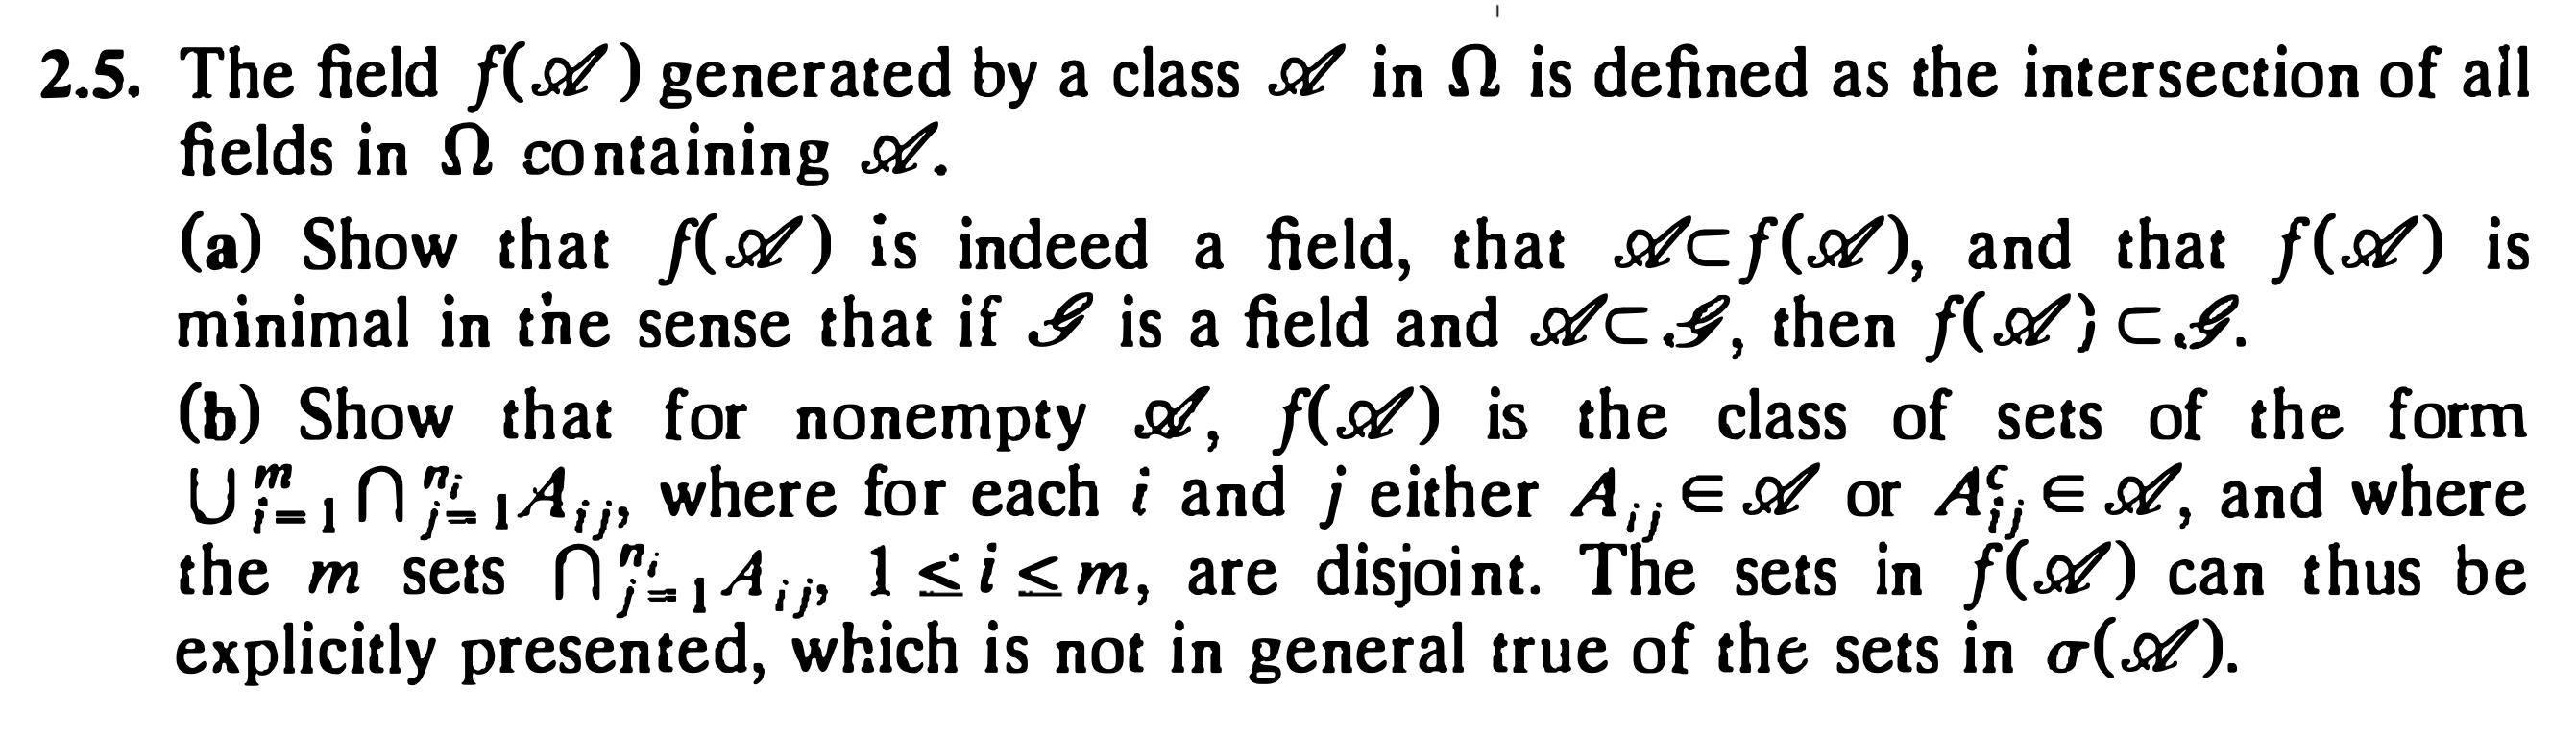
\includegraphics[width=400pt]{img/analysis--berkeley-202a-hw-ab18.png}
  \end{mdframed}
  Let $\ms F_1, \ms F_2, \ldots$ be the collection of all algebras in $\Omega$ for which $\ms A \subset \ms F_n$,
  so that $f(\ms A) = \bigcap_{n}\ms F_n$.

  \begin{enumerate}[label=(\alph*)]

  \item
    \begin{claim*}
      $f(\ms A)$is an algebra
    \end{claim*}
    \begin{proof}
      We must show that
      \begin{enumerate}
      \item $\Omega \in f(\ms A)$\\
        {\bf Proof:} $\Omega \in \ms F_n$ for all $n$, therefore $\Omega \in \bigcap_{n}\ms F_n = f(\ms A)$.

      \item If $X \in f(\ms A)$ then $X^c \in f(\ms A)$\\
        {\bf Proof:} If $X \in f(\ms A)$ then $X \in \ms F_n$ for all $n$, therefore $X^c \in \ms F_n$ for all $n$, therefore $X^c \in \bigcap_{n}\ms F_n = f(\ms A)$.

      \item If $X, Y \in f(\ms A)$ then $X \cup Y \in f(\ms A)$\\
        {\bf Proof:} If $X, Y \in f(\ms A)$ then $X, Y \in \ms F_n$ for all $n$, therefore $X \cup Y \in \ms F_n$ for all $n$, therefore $X \cup Y \in f(\ms A)$.
      \end{enumerate}
    \end{proof}

    \begin{claim*}
      $\ms A \subset f(\ms A)$
    \end{claim*}
    \begin{proof}
      Let $X \in \ms A$. Then $X \in \ms F_n$ for all $n$. Therefore $X \in \bigcap_{n}\ms F_n = f(\ms A)$. Therefore $\ms A \subset f(\ms A)$.
    \end{proof}

    \begin{claim*}
      $f(\ms A)$ is minimal in the sense that if $\ms G$ is an algebra and $\ms A \subset \ms G$, then $f(\ms A) \subset \ms G$.
    \end{claim*}
    \begin{proof}
      If $\ms G$ is an algebra with $\ms A \subset \ms G$ then $\ms G \in \{\ms F_1, \ms F_2, \ldots\}$, therefore $\ms G \supset \bigcap_{n}\ms F_n = f(\ms A)$.
    \end{proof}

  \item
    \red{TODO}

    [For (b) I looked at the hint in Billingsley and got hints from other students.]

    \begin{proof}
      Let $\ms B$ be the class of sets of the form $\bigcup_{i=1}^m \bigcap_{j=1}^{n_i} A_{ij}$, where
      either $A_{ij} \in \ms A$ or $A^c_{ij} \in \ms A$,
      with $\big\{\bigcap_{j=1}^{n_i} A_{ij} ~ : ~ i \in \{1, \ldots m\}\big\}$ disjoint.

      We want to show that $\ms B = f(\ms A)$. Note that $f(\ms A)$ is the smallest algebra containing $\ms A$.
      Therefore it suffices to show that $\ms B$ is a algebra and that $\ms B \subseteq f(\ms A)$.

      Let $B \in \ms B$. Then $B$ is formed from the elements of $\ms A$ by taking complements, finite unions
      and finite intersections. Therefore $B \in f(\ms A)$. Therefore $\ms B \subseteq f(\ms A)$.

      It remains to show that $\ms B$ is a algebra.

      Note that $\emptyset \in \ms B$, since with $m = n_1 = 1$ and $A_{11} = \emptyset$, we
      have $\emptyset = \bigcup_{i=1}^m\bigcap_{j=1}^{n_1}A_{ij}$.

      Next we show that $\ms B$ is closed under finite intersections.
      Let $B = \bigcup_{i=1}^m \bigcap_{j=1}^{n_i} A_{ij}$, where either $A_{ij} \in \ms A$
      or $A^c_{ij} \in \ms A$, and let $B' = \bigcup_{i=1}^{m'} \bigcap_{j=1}^{n'_i} A'_{ij}$, where
      either $A'_{ij} \in \ms A$ or $A^{'c}_{ij} \in \ms A$.

      We have
      \begin{align*}
        B \cap B'
        =& \big(\bigcup_{i=1}^m \bigcap_{j=1}^{n_i} A_{ij}\big)
           \bigcap
           \big(\bigcup_{i=1}^{m'} \bigcap_{j=1}^{n'_{i}} A'_{ij}\big)
      \end{align*}
      [\red{TODO} I think I should be able to simplify this from basic undergrad set theory and show that the result
      is of the desired form.]

      It follows from induction that $\ms B$ is closed under finite intersections.

      Finally we show that $\ms B$ is closed under complements. As before,
      let $B = \bigcup_{i=1}^m \bigcap_{j=1}^{n_i} A_{ij}$, where either $A_{ij} \in \ms A$
      or $A^c_{ij} \in \ms A$. Then
      \begin{align*}
        B^c
        &= \Big(\bigcup_{i=1}^m \bigcap_{j=1}^{n_i} A_{ij}\Big)^c \\
        &= \bigcap_{i=1}^m \bigcup_{j=1}^{n_i} A^c_{ij}.
      \end{align*}

      \red{TODO} Why is this of the required form?
    \end{proof}

  \end{enumerate}
  \newpage
\item~\\
  \begin{mdframed}
    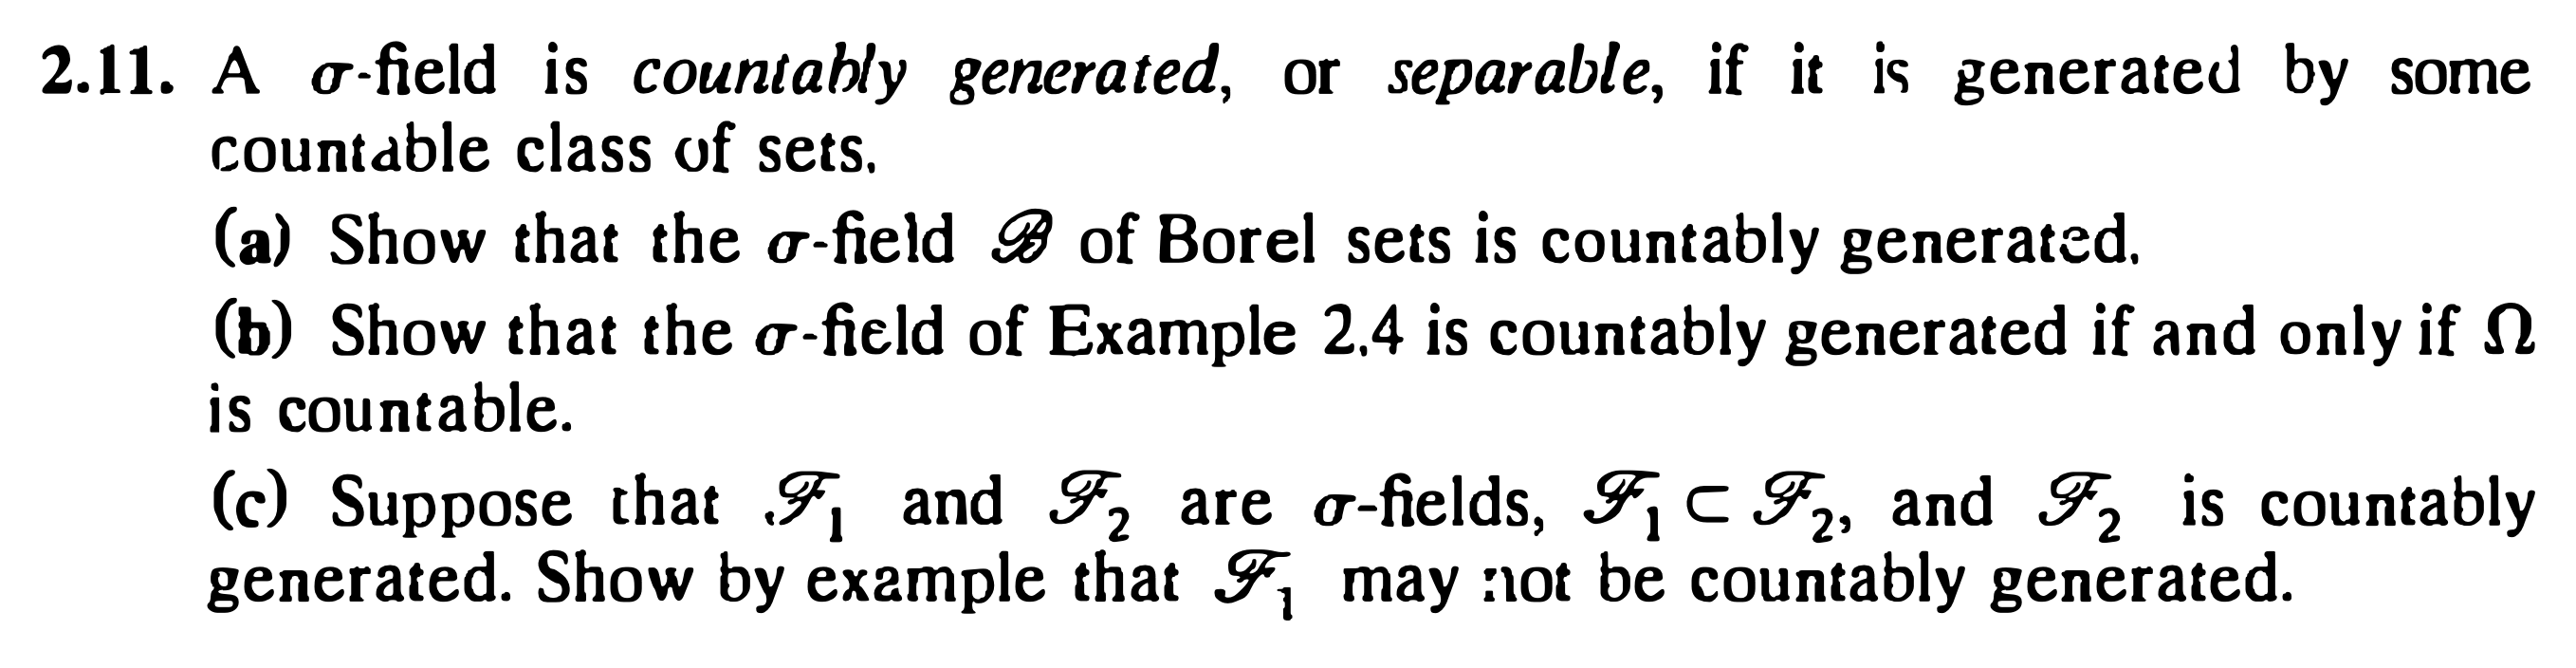
\includegraphics[width=400pt]{img/analysis--berkeley-202a-hw-fc85.png}
  \end{mdframed}
  \begin{definition*}
    Let $\Omega = (0, 1]$ and let $\ms O$ be the collection of open subsets of $\Omega$. Each element of the
    Borel $\sigma$-algebra $\ms B := \sigma(\ms O)$ is a Borel set.
  \end{definition*}

  \begin{lemma}\label{hw3-2-11-lemma-1}
    Let $\ms I_1 = \{(a, b) ~:~ a, b \in \R\}$. Then $\sigma(\ms I_1) = \ms B$.
  \end{lemma}
  \begin{proof}
    Let $\Omega = (0, 1]$ and let $\ms O$ be the collection of open subsets of $\Omega$.

    Let $\ms I_1 = \{(a, b) ~:~ a, b \in \R\}$. We want to show that $\sigma(\ms I_1) = \ms B := \sigma(\ms O)$.

    In one direction, every element of $\ms I_1$ is open, so clearly $\sigma(\ms I_1) \subseteq \sigma(\ms O)$.

    For the other direction, let $X \in \ms O$ be an open subset of $\R$. Then $X$ is a countable union of
    open intervals (i.e. finite intervals and open rays). Every finite interval is in $\ms I_1$. But an open
    ray is also a countable union of finite intervals: $(-\infty, a) = \bigcup_n^\infty (a-n, a)$
    and $(a, \infty) = \bigcup_n^\infty (a, a + n)$. Therefore $X \in \sigma(\ms I_1)$, i.e. every open set
    is in the $\sigma$-algebra generated by open intervals. This is equivalent to the
    statement $\ms O \subseteq \sigma(\ms I_1)$, i.e. the collection of all open sets is a subset of
    that $\sigma$-algebra. Therefore $\sigma(\ms O) \subseteq \sigma(\sigma(\ms I_1)) = \sigma(\ms I_1)$.
  \end{proof}

  \begin{enumerate}[label=(\alph*)]

  \item
    \begin{claim*}
      The $\sigma$-algebra $\ms B$ of Borel sets is countably generated.
    \end{claim*}
    \begin{proof}
      let $\ms O$ be the collection of open sets of $\Omega = (0, 1]$, so that $\ms B = \sigma(\ms O)$.

      Let $\ms I_1 = \{(a, b) ~:~ a, b \in \R\}$ and $\ms I_2 = \{(p, q) ~:~ p, q \in \Q\}$

      Note that $\ms I_2$ is a countable set (the rationals are countable, and any finite Cartesian product of
      countable sets is countable.)

      We claim that $\sigma(\ms I_2) = \sigma(\ms O)$.

      Inclusion in one direction is immediate, since $\ms I_2 \subset \ms O$ and
      therefore $\sigma(\ms I_2) \subseteq\sigma(\ms O)$.

      For inclusion in the other direction, note that for all $a, b \in \R$ with $a < b$
      \begin{align*}
        (a, b) = \bigcup_{\substack{p, q \in \Q\\a < p < q < b}} (p, q).
      \end{align*}
      Therefore $\sigma(\ms I_1) \subseteq \sigma(\ms I_2)$. But $\sigma(\ms I_1) = \sigma(\ms O)$ from lemma
      (\ref{hw3-2-11-lemma-1}) hence $\sigma(\ms O) \subseteq \sigma(\ms I_2)$.
    \end{proof}
  \item
    \begin{claim*}
      Let $\ms F$ be a $\sigma$-algebra containing the countable and cocountable subsets of $\Omega$ ($A$ being
      cocountable if $A^c$ is countable). Then $\ms F$ is countably generated if and only if $\Omega$ is
      countable.
    \end{claim*}
    \begin{proof}
      [Looked at hint in Billingsley and got hints from other students.]

      First let $\Omega$ be countable. We want to show that there exists a countable class of sets that
      generates $\ms F$. Indeed, the class of all singletons generates $\ms F$ and is countable.

      Next let $\Omega$ be uncountable. We want to show that every class of sets that generates $\ms F$ is
      uncountable.

      Suppose for a contradiction that $\ms F$ is countably generated and let $\ms A = \{A_1, A_2, \dots\}$ be
      a countable class of countable sets that generates $\ms F$. (We can stipulate that every element
      of $\ms A$ is countable since, if it is not, we may replace it with its complement, which is.)

      Let $\Omega_0 = \bigcup_i A_i$. Then $\Omega_0$ is countable
      and $\ms S_0 := \{\{\om\}: \om \in \Omega_0\}$ is a countable class of singletons. We see that $\ms A$ is
      generated by $\ms S_0$, and therefore that $\ms F$ is generated by $\ms S_0$.

      Now consider $\Omega^c_0$. We want to derive a contradiction, and presumably that contradiction is going
      to be concluding that $\Omega^c_0$ is countable when in fact we know it is uncountable, because $\Omega$
      is. \red{TODO}
    \end{proof}
  \end{enumerate}

  \newpage
\item~\\
  \begin{mdframed}
    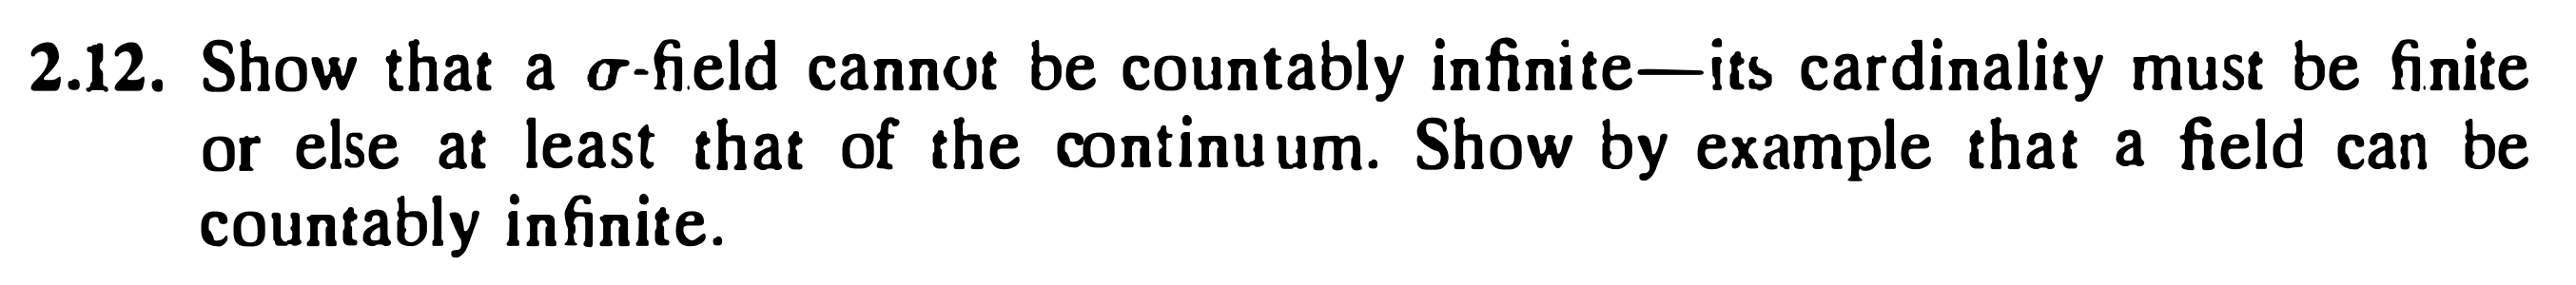
\includegraphics[width=400pt]{img/analysis--berkeley-202a-hw-af2a.png}
  \end{mdframed}
  \begin{claim*}
    A $\sigma$-algebra cannot be countably infinite.
  \end{claim*}
  \begin{proof}
    Let $\ms A$ be a non-finite $\sigma$-algebra on $\Omega$. If (\red{TODO}) we can show that $\ms A$ contains a
    countable set of singletons then we are done, because then $\ms A$ contains all subsets that can be formed
    from those singletons by countable unions, in which case its cardinality is at least $2^{\aleph_0}$.
  \end{proof}


  \begin{claim*}
    An algebra can be countably infinite.
  \end{claim*}

  \begin{proof}
    Let $\Omega$ be $\{1, 2, \ldots\}$. Build a collection of subsets $\ms A$ according to the following algorithm:

    Set $\ms A = \emptyset$\\
    For $i \in 1, 2, \dots$\\
    ...........For $A \in \mc P(\{1, \dots, n\})$\\
    ......................Set $\ms A = \ms A \cup \{A, A^c\}$

    Thus $\ms A$ contains every finite set, and its complement, and is countable by construction.
    Clearly $\ms A$ is closed under complements. To see that $\ms A$ is closed under finite unions,
    let $A_1, A_2 \in \ms A$. There are two cases:
    \begin{enumerate}
    \item Suppose one of $A_1, A_2$ is countably infinite. Then $A_1 \cup A_2$ is countably infinite and is the complement of
      some finite set $(A_1 \cup A_2)$.
    \item Alternatively suppose both are finite. Then $A_1 \cup A_2$ is finite.
    \end{enumerate}
    In both cases, $A_1 \cup A_2 \in \ms A$ and $(A_1 \cup A_2)^c \in \ms A$. It follows by induction
    that $\ms A$ is closed under finite unions.
  \end{proof}
  \newpage
\item~\\
  \begin{mdframed}
    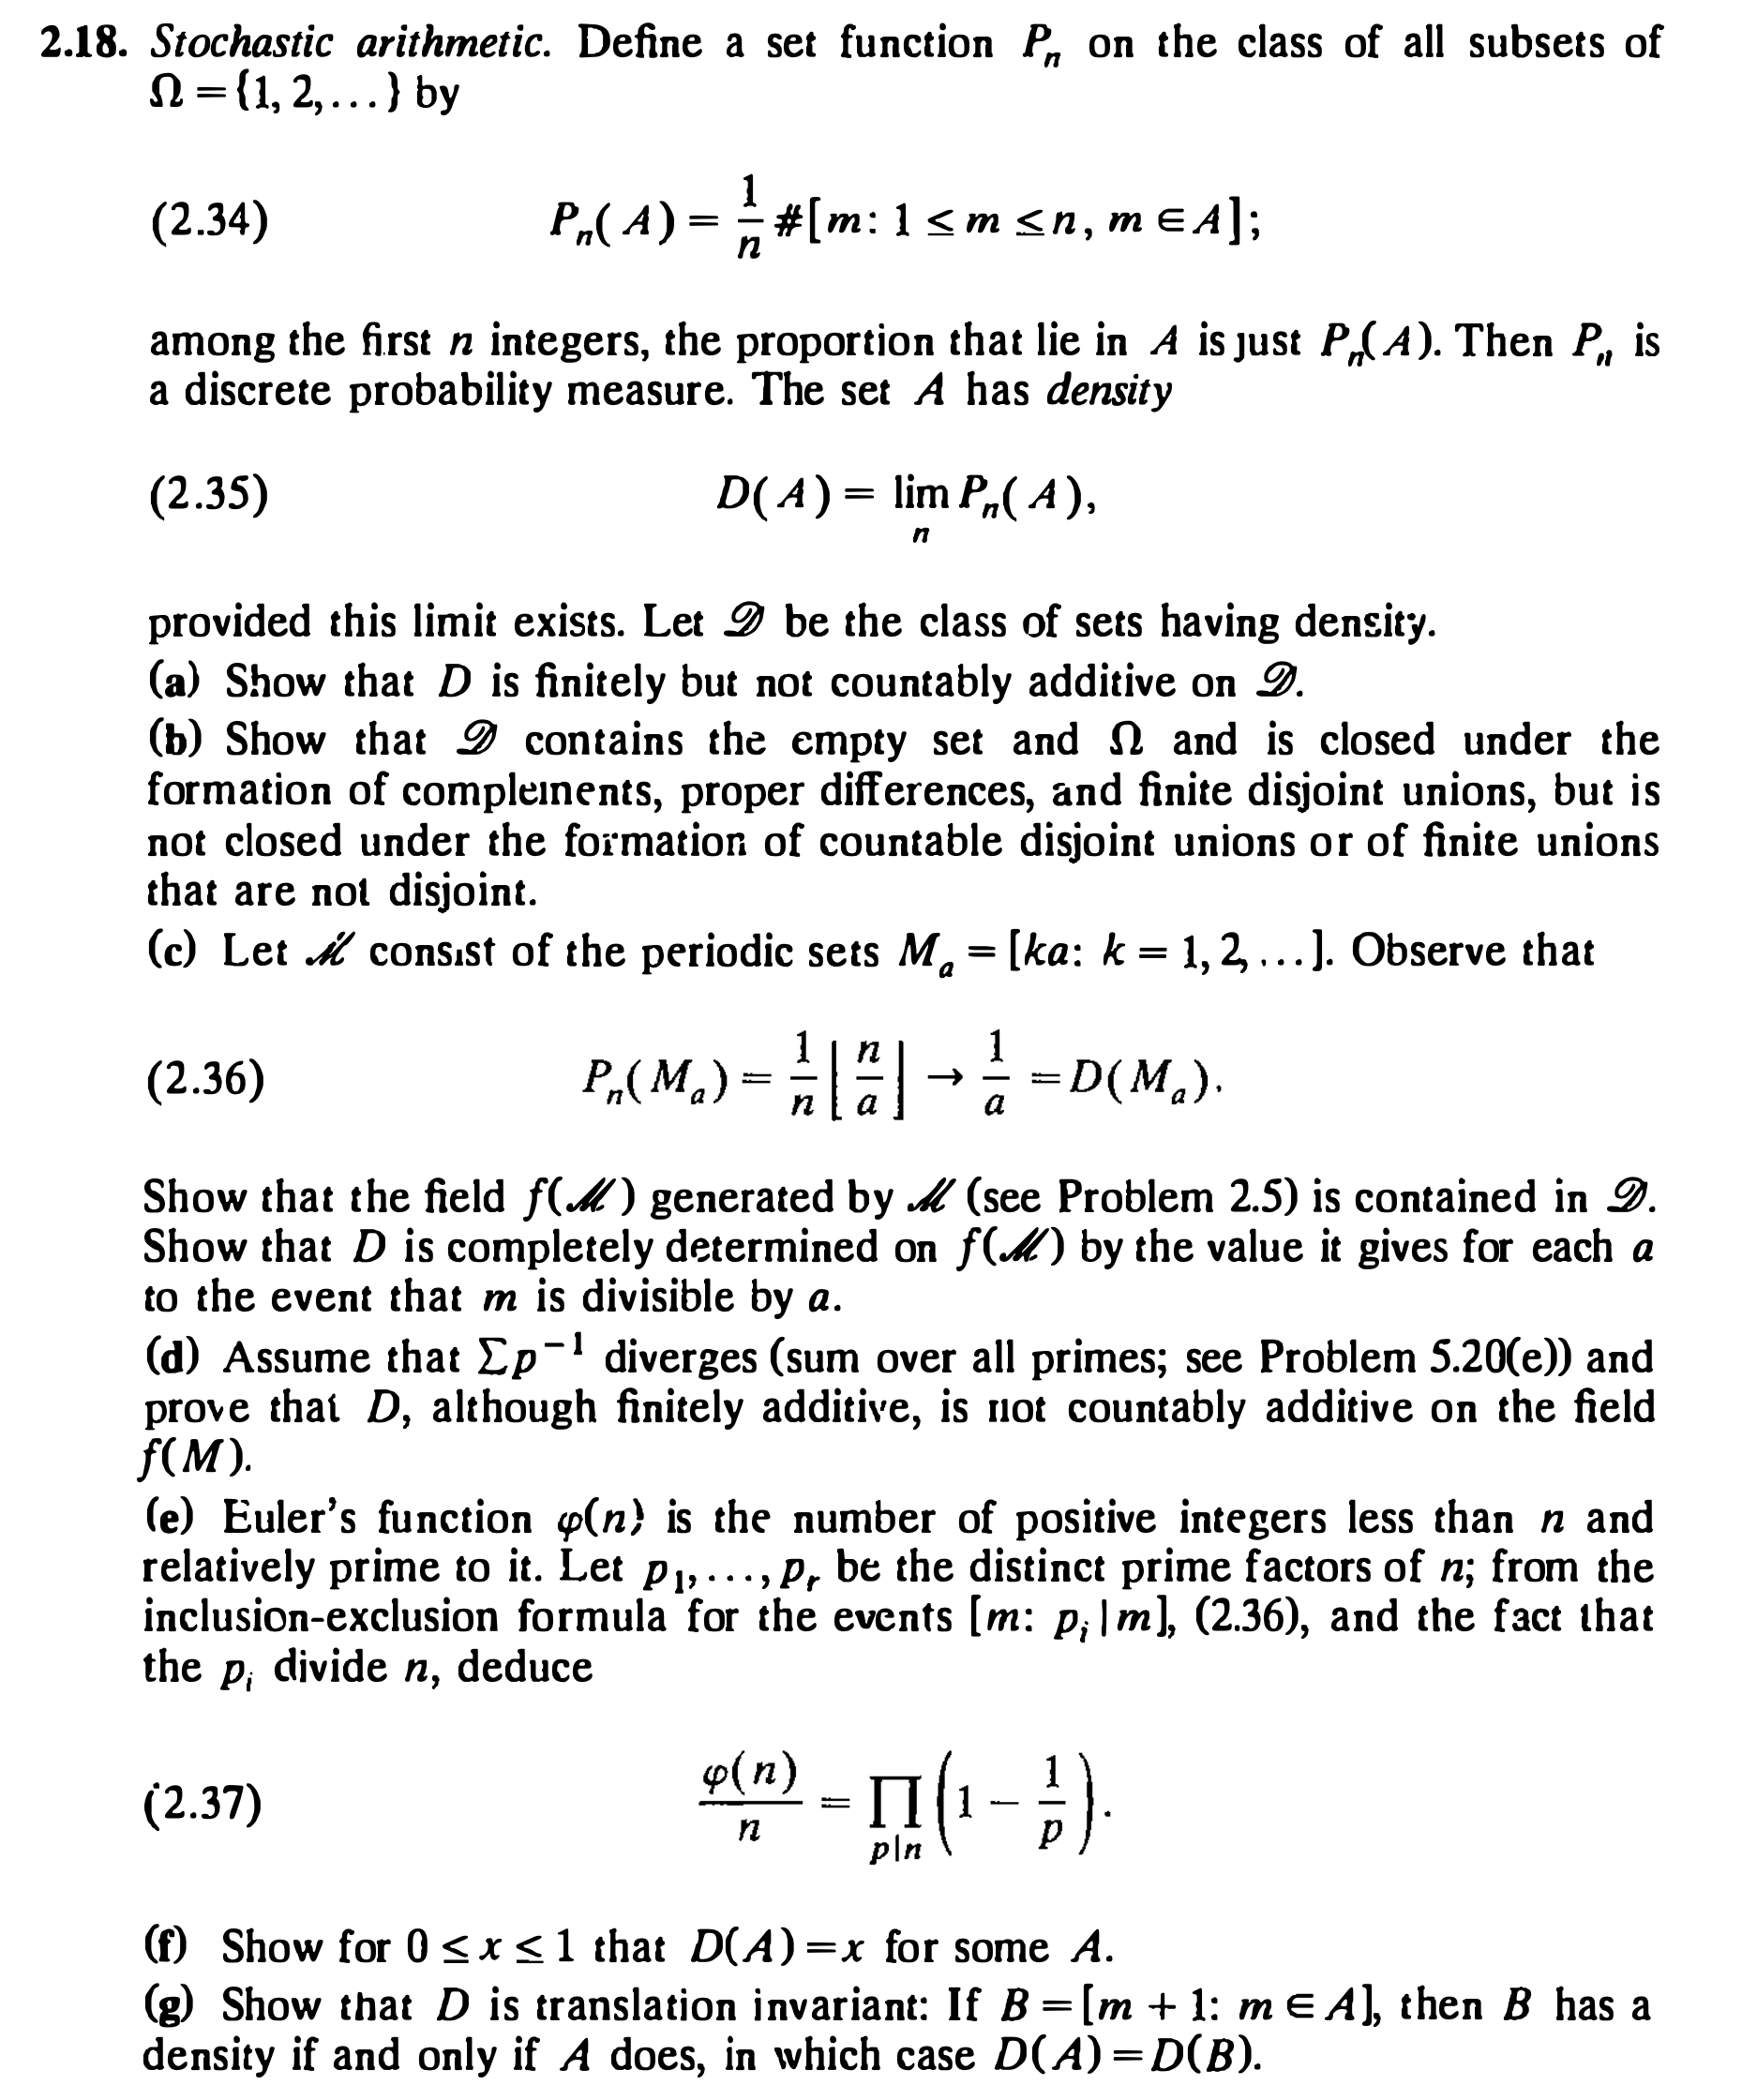
\includegraphics[width=400pt]{img/analysis--berkeley-202a-hw-b476.png}
  \end{mdframed}

  \begin{enumerate}[label=(\alph*)]

  \item
    \begin{claim*}
      $D$ is finitely but not countably additive on $\ms D$.
    \end{claim*}
    \begin{proof}
      Let $A_1$ and $A_2$ be disjoint subsets of $\Omega = \{1, 2, \ldots\}$. Then
      \begin{align*}
        D(A_1 \cup A_2)
        &= \lim_{n\to\infty} \big|\big\{m ~:~ 1 \leq m \leq n, m \in A_1 \cup A_2 \big\}\big| \\
        &= \lim_{n\to\infty} \big|\big\{m ~:~ 1 \leq m \leq n, m \in A_1 \big\} \bigcup \big\{m ~:~ 1 \leq m \leq n, m \in A_2 \big\}\big|\\
        &= \lim_{n\to\infty} \big|\big\{m ~:~ 1 \leq m \leq n, m \in A_1 \big\}\big| + \big|\big\{m ~:~ 1 \leq m \leq n, m \in A_2 \big\}\big| \\
        &= \lim_{n\to\infty} \big|\big\{m ~:~ 1 \leq m \leq n, m \in A_1 \big\}\big| + \lim_{n\to\infty} \big|\big\{m ~:~ 1 \leq m \leq n, m \in A_2 \big\}\big| \\
        &= D(A_1) + D(A_2).
      \end{align*}
      Finite additivity then follows by induction.

      To show that $\ms D$ is not countably additive, it is sufficient to provide a counter-example.

      Let $A_i = \{i\}$ for all $i \in \{1, 2, \ldots\}$ and let $\ms A = \bigcup_{i=1}^\infty A_i$ be the collection of all the singleton sets.

      Note that $D(A_i) = 0$ for all $i$. However $\bigcup_{i=1}^\infty A_i = \N$ and
      therefore $D\big(\bigcup_{i=1}^\infty A_i\big) = 1$. Therefore $D$ is not countably additive, since
      \begin{align*}
        \sum_{i=1}^\infty D(A_i) = \sum_{i=1}^\infty 0 = 0 \neq 1 = D\big(\bigcup_{i=1}^\infty A_i\big).
      \end{align*}
    \end{proof}

  \item
    \begin{enumerate}
    \item
      \begin{claim*}
        $\ms D$ contains $\emptyset$ and $\Omega$.
      \end{claim*}
      \begin{proof}
        $P_n(\emptyset) = 0$ for all $n$, therefore the limit exists and
        is $D(\emptyset) := \lim_{n\to\infty} 0 = 0$, therefore $\emptyset \in \ms D$.

        $P_n(\Omega) = 1$ for all $n$, therefore the limit exists and
        is $D(\Omega) := \lim_{n\to\infty} 1 = 1$, therefore $\Omega \in \ms D$.
      \end{proof}
    \item
      \begin{claim*}
        $\ms D$ is closed under complementation, proper differences, and finite disjoint unions.
      \end{claim*}
      \begin{proof}
        \begin{enumerate}
        \item {\bf Complementation}\\
          Let $A \in \ms D$. Then $A^c \in \ms D$ since $\ms D(A^c) = \lim_n P_n(A^c)$ exists and
          is $\ms D(A^c) = \lim_n P_n(A^c) = \lim_n (1 - P_n(A)) = 1 - D(A)$.
        \item {\bf Proper differences}\\
          Let $A_1, A_2 \in \ms D$ with $A_1 \subset A_2$. Then $A_2 \setminus A_1 \in \ms D$ since the limit exists:
          \begin{align*}
            D(A_2 \setminus A_1) = \lim_n (P_n(A_2 \setminus A_1)) = \lim_n P_n(A_2) - \lim_nP_n(A_1) = D(A_2) - D(A_1).
          \end{align*}
        \item {\bf Finite disjoint unions}\\
          Let $A_1, A_2 \in \ms D$. Then $A_1 \cup A_2 \in \ms D$ since the limit exists:
          \begin{align*}
            D(A_1 \cup A_2) = \lim_n (P_n(A_1) + P_n(A_2)) = \lim_n P_n(A_1) + \lim_n  P_n(A_2)) = D(A_2) + D(A_1).
          \end{align*}
        \end{enumerate}
      \end{proof}
    \item
      \begin{claim*}
        $\ms D$ is not closed under countable disjoint unions.
      \end{claim*}
      \begin{proof}
        An example of a subset of $\{1, 2, \ldots\}$ that has no density is the set of positive integers whose
        binary representation has an odd number of digits. This can be formed as a countable union of disjoint
        sets: (one-digit) $\bigcup$ (three-digits) $\bigcup \ldots$.

        Informally, this set consists of a stretch of consecutive integers that are included, followed by a
        longer stretch that are excluded, followed by a longer still stretch that are included, and so on. The
        reason there is no limiting density is that the density fluctuates, and the way in which the stretches
        increase in length means that the amplitude of the density fluctuations does not decrease to zero.

        \red{TODO} prove that $D(A) := \lim_{n\to\infty} P_n(A)$ does not exist.
      \end{proof}
    \item
      \begin{claim*}
        $\ms D$ is not closed under finite unions that are not disjoint.
      \end{claim*}
    \end{enumerate}

  \item
    \begin{claim*}
       $f(\ms M)$ is contained in $\ms D$.
    \end{claim*}
    \begin{proof}

      [NOT ATTEMPTED]
    \end{proof}
    \begin{claim*}
      $D$ is completely determined on $f(\ms M)$ by the value it gives for each $a$ to the event that $m$ is
      divisible by $a$.

      In other words:

      Let $A \in f(\ms M)$. Then $D(A)$ can be computed knowing only the values $D(M_1), D(M_2), D(M_3), \ldots$.
    \end{claim*}
    \begin{proof}

      [NOT ATTEMPTED]
    \end{proof}

  \item
    \begin{claim*}
      $D$ is finitely additive but not countably additive on $f(\ms M)$.
    \end{claim*}
    \begin{proof}

      [INCOMPLETE]

      For $n \geq 2$ define
      \begin{align*}
        L_n = M_n \setminus \bigcup_{2 \leq i < n} M_i.
      \end{align*}
      Note that
      \begin{align*}
        D(L_2) &= 1/2 \\
        D(L_3) &< 1/3 \\
        D(L_4) &= 0 \\
        D(L_5) &< 1/5 \\
        D(L_6) &= 0 \\
        D(L_7) &< 1/7 \\
        D(L_8) &= 0 \\
        \vdots
      \end{align*}
      The $L_n$ are disjoint, and we have $D(\bigcup_{n \geq 2} L_n) = D(\{2, \ldots\}) = 1$.

      We want to show that $\sum_n D(L_n) \neq 1$ but that is not clear: it is given that the sum of the
      reciprocals of the primes diverges, but our sum is smaller than that.

      \red{TODO}
    \end{proof}

  \item
    \begin{claim*}
      Let $\varphi(n)$ be Euler's function. Then
      \begin{align*}
        \frac{\varphi(n)}{n} = \prod_{p|n}\big(1 - \frac{1}{p}\big).
      \end{align*}
    \end{claim*}
    \begin{proof}

      [INCOMPLETE]

      Fix $n \in \{1, 2, \ldots\}$ and let $p_1, \ldots, p_r$ be the distinct prime factors of $n$, so that $n = \prod_{i=1}^rp_i^{k_i}$.
      Then
      \begin{align*}
        \frac{\varphi(n)}{n} &= \frac{\#\big\{i ~:~ 1 \leq i < n, i \text{~coprime with~} n\big\}}{n} \\
                             &= \frac{(n - 1) - \#\big\{i ~:~ 1 \leq i < n, i \text{~is a multiple of~} p_j \text{~for some~} 1 \leq j \leq r\big\}}{n} \\
                             &= \frac{(n - 1) - \#\big\{i ~:~ 1 \leq i < n, i \in \bigcup_{j=1}^r M_{p_j}\big\}}{n} \\
      \end{align*}
      Fix $n \in \{1, 2, \ldots\}$ and let $p_1, \ldots, p_r$ be the distinct prime factors of $n$.
      Then
      \begin{align*}
        \varphi(n)
        &= n P_n\Big(\big(\bigcup_{i=1}^r M_p\big)^c\Big) \\
        &= n \Big(1 - P_n\big(\bigcup_{i=1}^r M_p\big)\Big) \\
        &= n \Big(1 - \Big(\frac{1}{p_1} + \frac{1}{p_2} + \frac{1}{p_3} + \ldots - \frac{1}{p_1p_2} - \frac{1}{p_1p_3} - \ldots + (-1)^r\frac{1}{p_1p_2p_3\cdots p_r}\Big)\Big) \\
        &= n \prod_{i=1}^r(1 - p_i).
      \end{align*}
    \end{proof}

  \item
    \begin{claim*}
	    $D(A) = x$ has a solution for all $0 \leq x \leq 1$.
    \end{claim*}
    \begin{proof}

      [INCOMPLETE]

      A set $A$ with density $ 0 \leq x \leq 1$ can be constructed by finding a series
      \begin{align*}
        \sum_{i=1}^\infty D(A_i)
      \end{align*}
      that converges to $x$ where the $A_i$ are disjoint elements of an algebra on which $D$ is countably
      additive.

      But we haven't yet identified any algebra on which $D$ is countably additive.
    \end{proof}

  \item
    \begin{claim*}
      $D$ is translation invariant.
    \end{claim*}
    \begin{proof}

      [NOT ATTEMPTED]
    \end{proof}
  \end{enumerate}
  [Note that a in part (c) is a positive integer.]

\end{enumerate}
